\documentclass{beamer}
\usepackage[utf8]{inputenc}
\usepackage{graphicx, epsfig}
\usepackage{amsmath,mathrsfs,amsfonts,amssymb}
\usepackage{floatflt}
\usepackage{epic,ecltree}
\usepackage{mathtext}
\usepackage{fancybox}
\usepackage{fancyhdr}
\usepackage{multirow}
\usepackage{enumerate}
\usepackage{epstopdf}
\usepackage{multicol}
\usepackage{algorithm}
\usepackage[noend]{algorithmic}
\usepackage{tikz}
\usepackage{blindtext}
\usetheme{default}%{Singapore}%{Warsaw}%{Warsaw}%{Darmstadt}
\usecolortheme{default}

\setbeamerfont{title}{size=\Huge}
\setbeamertemplate{footline}[page number]{}

\setbeamertemplate{section in toc}[sections numbered]


\makeatletter
\newcommand\HUGE{\@setfontsize\Huge{35}{40}}
\makeatother    

\setbeamerfont{title}{size=\HUGE}
\beamertemplatenavigationsymbolsempty

% latin bold lower
\newcommand{\ba}{\mathbf{a}} 
\newcommand{\bc}{\mathbf{c}} 
\newcommand{\be}{\mathbf{e}} 
\newcommand{\bh}{\mathbf{h}} 
\newcommand{\bp}{\mathbf{p}} 
\newcommand{\bt}{\mathbf{t}} 
\newcommand{\bs}{\mathbf{s}} 
\newcommand{\bu}{\mathbf{u}} 
\newcommand{\bv}{\mathbf{v}} 
\newcommand{\bw}{\mathbf{w}} 
\newcommand{\bx}{\mathbf{x}} 
\newcommand{\by}{\mathbf{y}} 
\newcommand{\bz}{\mathbf{z}} 

% latin bold upper
\newcommand{\bA}{\mathbf{A}} 
\newcommand{\bB}{\mathbf{B}} 
\newcommand{\bC}{\mathbf{C}} 
\newcommand{\bI}{\mathbf{I}} 
\newcommand{\bJ}{\mathbf{J}} 
\newcommand{\bL}{\mathbf{L}} 
\newcommand{\bM}{\mathbf{M}} 
\newcommand{\bP}{\mathbf{P}}
\newcommand{\bQ}{\mathbf{Q}} 
\newcommand{\bR}{\mathbf{R}} 
\newcommand{\bT}{\mathbf{T}} 
\newcommand{\bU}{\mathbf{U}} 
\newcommand{\bV}{\mathbf{V}} 
\newcommand{\bW}{\mathbf{W}} 
\newcommand{\bX}{\mathbf{X}} 
\newcommand{\bY}{\mathbf{Y}} 
\newcommand{\bZ}{\mathbf{Z}} 

% latin cal upper
\newcommand{\cF}{\mathcal{F}} 
\newcommand{\cG}{\mathcal{G}} 
\newcommand{\cI}{\mathcal{I}} 
\newcommand{\cL}{\mathcal{L}} 
\newcommand{\cM}{\mathcal{M}} 
\newcommand{\cN}{\mathcal{N}} 
\newcommand{\cP}{\mathcal{P}} 
\newcommand{\cS}{\mathcal{S}} 
\newcommand{\cT}{\mathcal{T}} 
\newcommand{\cW}{\mathcal{W}} 
\newcommand{\cX}{\mathcal{X}} 
\newcommand{\cZ}{\mathcal{Z}} 

% latin bb upper
\newcommand{\bbE}{\mathbb{E}} 
\newcommand{\bbI}{\mathbb{I}} 
\newcommand{\bbP}{\mathbb{P}} 
\newcommand{\bbR}{\mathbb{R}} 

% greek bold lower
\newcommand{\bepsilon}{\boldsymbol{\epsilon}} 
\newcommand{\btheta}{\boldsymbol{\theta}} 
\newcommand{\blambda}{\boldsymbol{\lambda}} 
\newcommand{\bpi}{\boldsymbol{\pi}} 
\newcommand{\bmu}{\boldsymbol{\mu}} 
\newcommand{\bsigma}{\boldsymbol{\sigma}} 
\newcommand{\bphi}{\boldsymbol{\phi}} 

% greek bold upper
\newcommand{\bSigma}{\boldsymbol{\Sigma}} 

\DeclareMathOperator*{\argmin}{arg\,min}
\DeclareMathOperator*{\argmax}{arg\,max}

\newcommand{\createdgmtitle}[1]{\title[\hbox to 56mm{Deep Generative Models  \hfill\insertframenumber\,/\,\inserttotalframenumber}]
	{\vspace{1cm} \\ \textbf{Deep Generative Models} \\ {\Huge Lecture #1}}
	\author{Roman Isachenko}
		\institute{
\includegraphics[width=0.7cm]{../utils/aimasterslogo} \LARGE{AI Masters}}
	\date{2024, Spring}
}

\usepackage{tikz}
\usetikzlibrary{arrows,shapes,positioning,shadows,trees}

\newcommand\myfootnote[1]{%
  \tikz[remember picture,overlay]
  \draw (current page.south west) +(1in + \oddsidemargin,0.5em)
  node[anchor=south west,inner sep=0pt]{\parbox{\textwidth}{%
      \rlap{\rule{10em}{0.4pt}}\raggedright\scriptsize \textit{#1}}};}

\newcommand\myfootnotewithlink[2]{%
  \tikz[remember picture,overlay]
  \draw (current page.south west) +(1in + \oddsidemargin,0.5em)
  node[anchor=south west,inner sep=0pt]{\parbox{\textwidth}{%
      \rlap{\rule{10em}{0.4pt}}\raggedright\scriptsize\href{#1}{\textit{#2}}}};}
      
\AtBeginSection[]
      {
      	\begin{frame}{Outline}
      		\tableofcontents[currentsection]
      	\end{frame}
      }
      \AtBeginSubsection[]{
      	\begin{frame}{Outline}
      		\tableofcontents[currentsection,currentsubsection]
      	\end{frame}
}
\createdgmtitle{10}

\usepackage{tikz}

\usetikzlibrary{arrows,shapes,positioning,shadows,trees}
%--------------------------------------------------------------------------------
\begin{document}
%--------------------------------------------------------------------------------
\begin{frame}[noframenumbering,plain]
%\thispagestyle{empty}
\titlepage
\end{frame}
%=======
\begin{frame}{Recap of previous lecture}
	Let take some pretrained image classification model to get the conditional label distribution $p(y | \bx)$ (e.g. ImageNet classifier).
	\begin{block}{Evaluation of likelihood-free models}
		\begin{itemize}
			\item Sharpness $\Rightarrow$ low $H(y | \bx) = - \sum_{y} \int_{\bx} p(y, \bx) \log p(y | \bx) d\bx$.
			\item Diversity $\Rightarrow$ high $H(y)  = - \sum_{y} p(y) \log p(y)$.
		\end{itemize}
	\end{block}
	\vspace{-0.3cm}
	\begin{block}{Inception Score}
		\vspace{-0.2cm}
		\[
			IS = \exp(H(y) - H(y | \bx)) = \exp \left( \bbE_{\bx} KL(p(y | \bx) || p(y)) \right)
		\]
		\vspace{-0.5cm}
	\end{block}
	\begin{block}{Frechet Inception Distance}
		\vspace{-0.3cm}
		\[
			D^2 (\pi, p) = \| \mathbf{m}_{\pi} - \mathbf{m}_{p}\|_2^2 + \text{Tr} \left( \bSigma_{\pi} + \bSigma_p - 2 \sqrt{\bSigma_{\pi} \bSigma_p} \right).
		\]
		\vspace{-0.5cm}
	\end{block}
	FID is related to moment matching.
	
	\myfootnote{\href{https://arxiv.org/abs/1606.03498}{Salimans T. et al. Improved Techniques for Training GANs, 2016} \\
	\href{https://arxiv.org/abs/1706.08500}{Heusel M. et al. GANs Trained by a Two Time-Scale Update Rule Converge to a Local Nash Equilibrium, 2017} }
\end{frame}
%=======
\begin{frame}{Recap of previous lecture}
		\begin{itemize}
			\item $\cS_{\pi} = \{\bx_i\}_{i=1}^{n} \sim \pi(\bx)$ -- real samples;
			\item $\cS_{p} = \{\bx_i\}_{i=1}^{n} \sim p(\bx | \btheta)$ -- generated samples.
		\end{itemize}
		Embed samples using pretrained classifier network (as previously):
		\[
			\cG_{\pi} = \{\mathbf{g}_i\}_{i=1}^n, \quad \cG_{p} = \{\mathbf{g}_i\}_{i=1}^n.
		\]
		Define binary function:
		\[
			f(\mathbf{g}, \cG) = 
			\begin{cases}
				1, \text{if exists } \mathbf{g}' \in \cG: \| \mathbf{g}  - \mathbf{g}'\|_2 \leq \| \mathbf{g}' - \text{NN}_k(\mathbf{g}', \cG)\|_2; \\
				0, \text{otherwise.}
			\end{cases}
		\]
		\[
			\text{Precision} (\cG_{\pi}, \cG_{p}) = \frac{1}{n} \sum_{\mathbf{g} \in \cG_{p}} f(\mathbf{g}, \cG_{\pi}); \quad \text{Recall} (\cG_{\pi}, \cG_{p}) = \frac{1}{n} \sum_{\mathbf{g} \in \cG_{\pi}} f(\mathbf{g}, \cG_{p}).
		\]
		\vspace{-0.4cm}
		\begin{figure}
			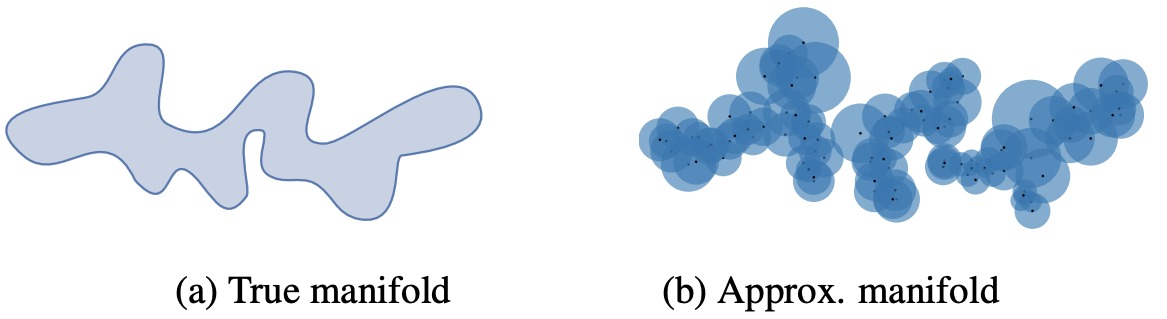
\includegraphics[width=0.7\linewidth]{figs/pr_k_nearest}
		\end{figure}
		\myfootnotewithlink{https://arxiv.org/abs/1904.06991}{Kynkäänniemi T. et al. Improved precision and recall metric for assessing generative models, 2019}
\end{frame}
%=======
\begin{frame}{Outline}
	\tableofcontents
\end{frame}
%=======
\section{Langevin dynamic}
%=======
\begin{frame}{Langevin dynamic}
	\vspace{-0.4cm}
	\begin{block}{Statement}
		Let $\bx_0$ be a random vector. Then samples from the following dynamics
		\vspace{-0.3cm}
		\[
			\bx_{t + 1} = \bx_t + \eta \frac{1}{2} \nabla_{\bx_t} \log p(\bx_t | \btheta) + \sqrt{\eta} \cdot \bepsilon, \quad \bepsilon \sim \cN(0, \bI).
		\]
		will come from $p(\bx | \btheta)$ under mild regularity conditions for small enough $\eta$ and large enough $t$.
	\end{block}
	\begin{minipage}{0.55\linewidth}
		\begin{itemize}
			\item Here we assume that we already have some generative model $p(\bx | \btheta)$.
			\item The density $p(\bx | \btheta)$ is a \textbf{stationary} distribution for this SDE. \\
			\item What do we get if $\bepsilon = \boldsymbol{0}$?
		\end{itemize}
	\end{minipage}%
	\begin{minipage}{0.4\linewidth}
		\begin{figure}
			\centering
			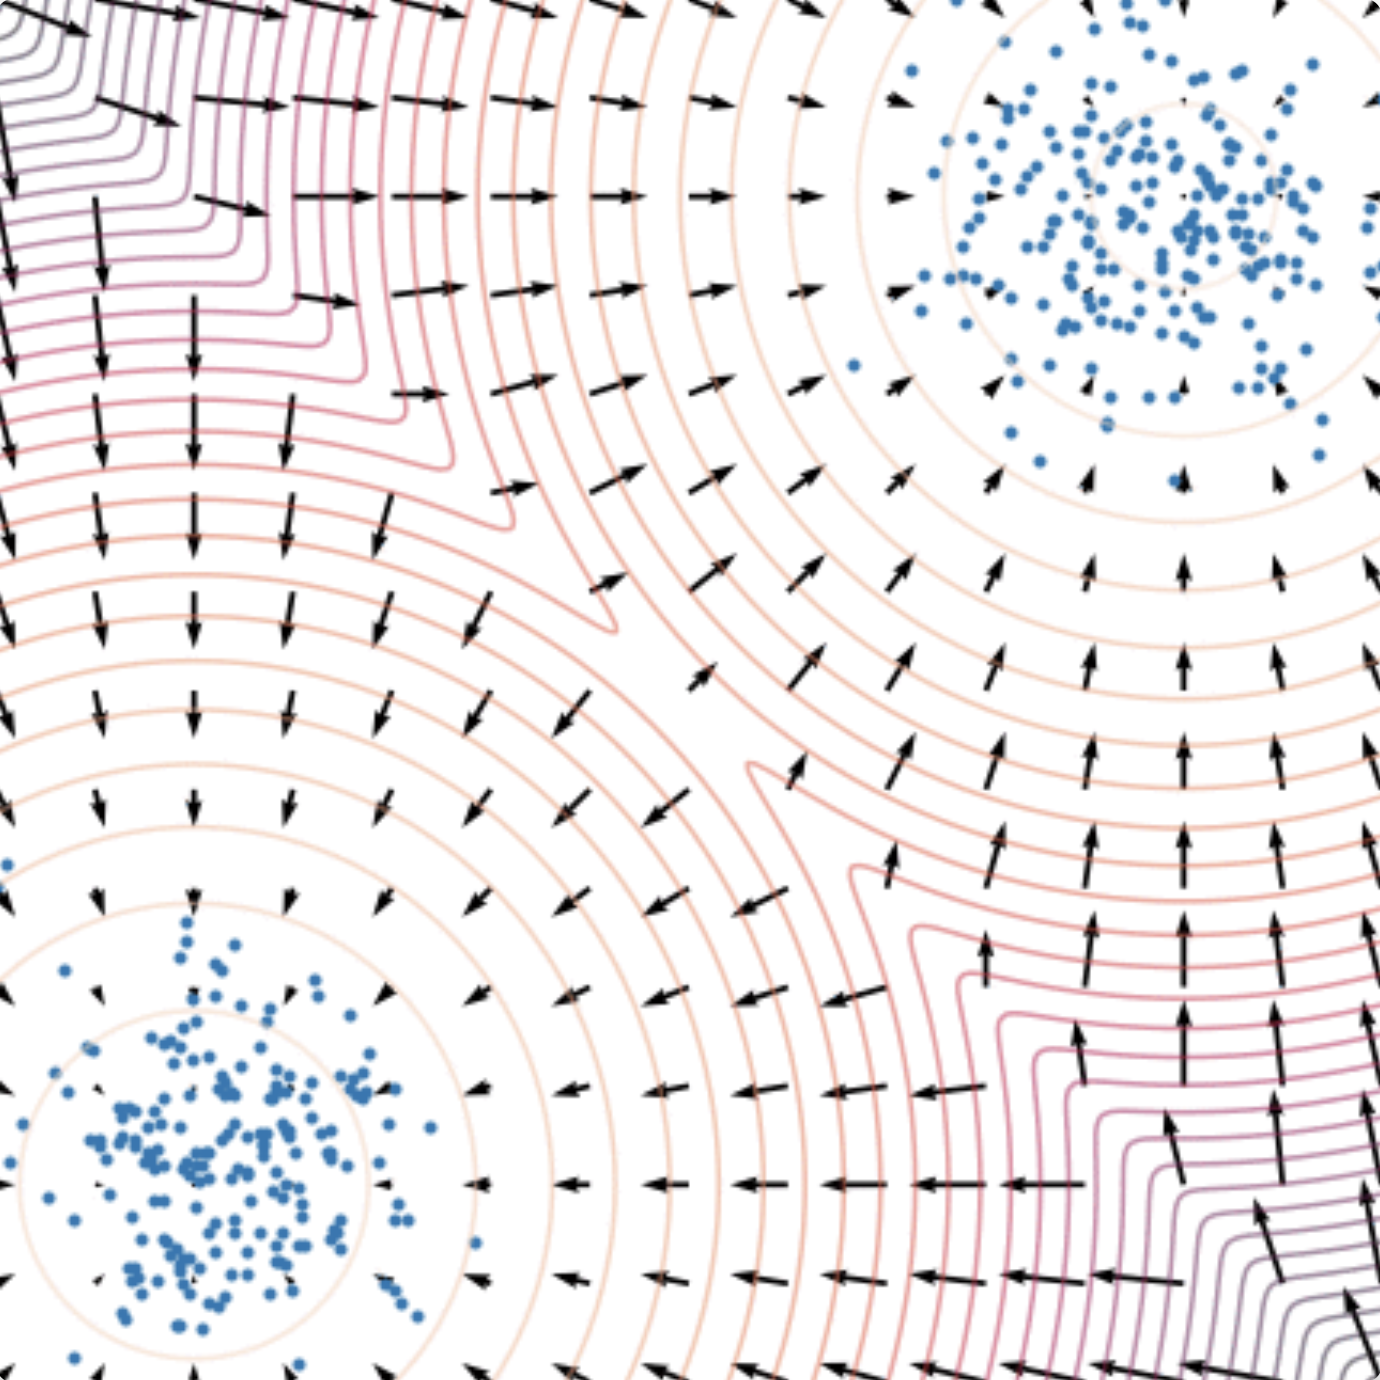
\includegraphics[width=0.9\linewidth]{figs/langevin_dynamic}
		\end{figure}
	\end{minipage}
	\myfootnotewithlink{https://yang-song.github.io/blog/2021/score/}{Song Y. Generative Modeling by Estimating Gradients of the Data Distribution, blog post, 2021} 
	\end{frame}
%=======
\begin{frame}{Energy-based models}
	\begin{itemize}
		\item We could sample from the model using Langevin dynamics if we have $\nabla_{\bx}\log p(\bx| \btheta)$.
		\item Where is it helpful?
	\end{itemize}
	\begin{block}{Unnormalized density}
		\vspace{-0.2cm}
		\[
			p(\bx | \btheta) = \frac{\hat{p}(\bx | \btheta)}{Z_{\btheta}}, \quad \text{where } Z_{\btheta} = \int \hat{p}(\bx | \btheta) d \bx
		\]
		\begin{itemize}
			\item $\hat{p}(\bx | \btheta)$ is any non-negative function. \\
			\item If we use the reparametrization $\hat{p}(\bx | \btheta) = \exp(-f_{\btheta}(\bx))$, we remove the non-negativite constraint.
		\end{itemize}
		\[
			\nabla_{\bx} \log p(\bx | \btheta) = \nabla_{\bx} \log \hat{p}(\bx | \btheta) - \nabla_{\bx} \log Z_{\btheta} = \nabla_{\bx} \log \hat{p}(\bx | \btheta)
		\]
		The gradient of the normalized density equals to the gradient of the unnormalized density.
	\end{block}
\end{frame}
%=======
\begin{frame}{Score matching}
	We could sample from the model using Langevin dynamics if we have $\nabla_{\bx}\log p(\bx| \btheta)$.
	\begin{block}{Fisher divergence}
		\vspace{-0.3cm}
		\[
		D_F(\pi, p) = \frac{1}{2}\bbE_{\pi}\bigl\| \nabla_{\bx}\log p(\bx| \btheta) - \nabla_\bx \log \pi(\bx) \bigr\|^2_2 \rightarrow \min_{\btheta}
		\]
		\vspace{-0.5cm}
	\end{block}
	Let introduce \textbf{score function} $\bs_{\btheta}(\bx) = \nabla_{\bx}\log p(\bx| \btheta)$. 
	\vspace{-0.2cm}
	\begin{figure}
		\centering
		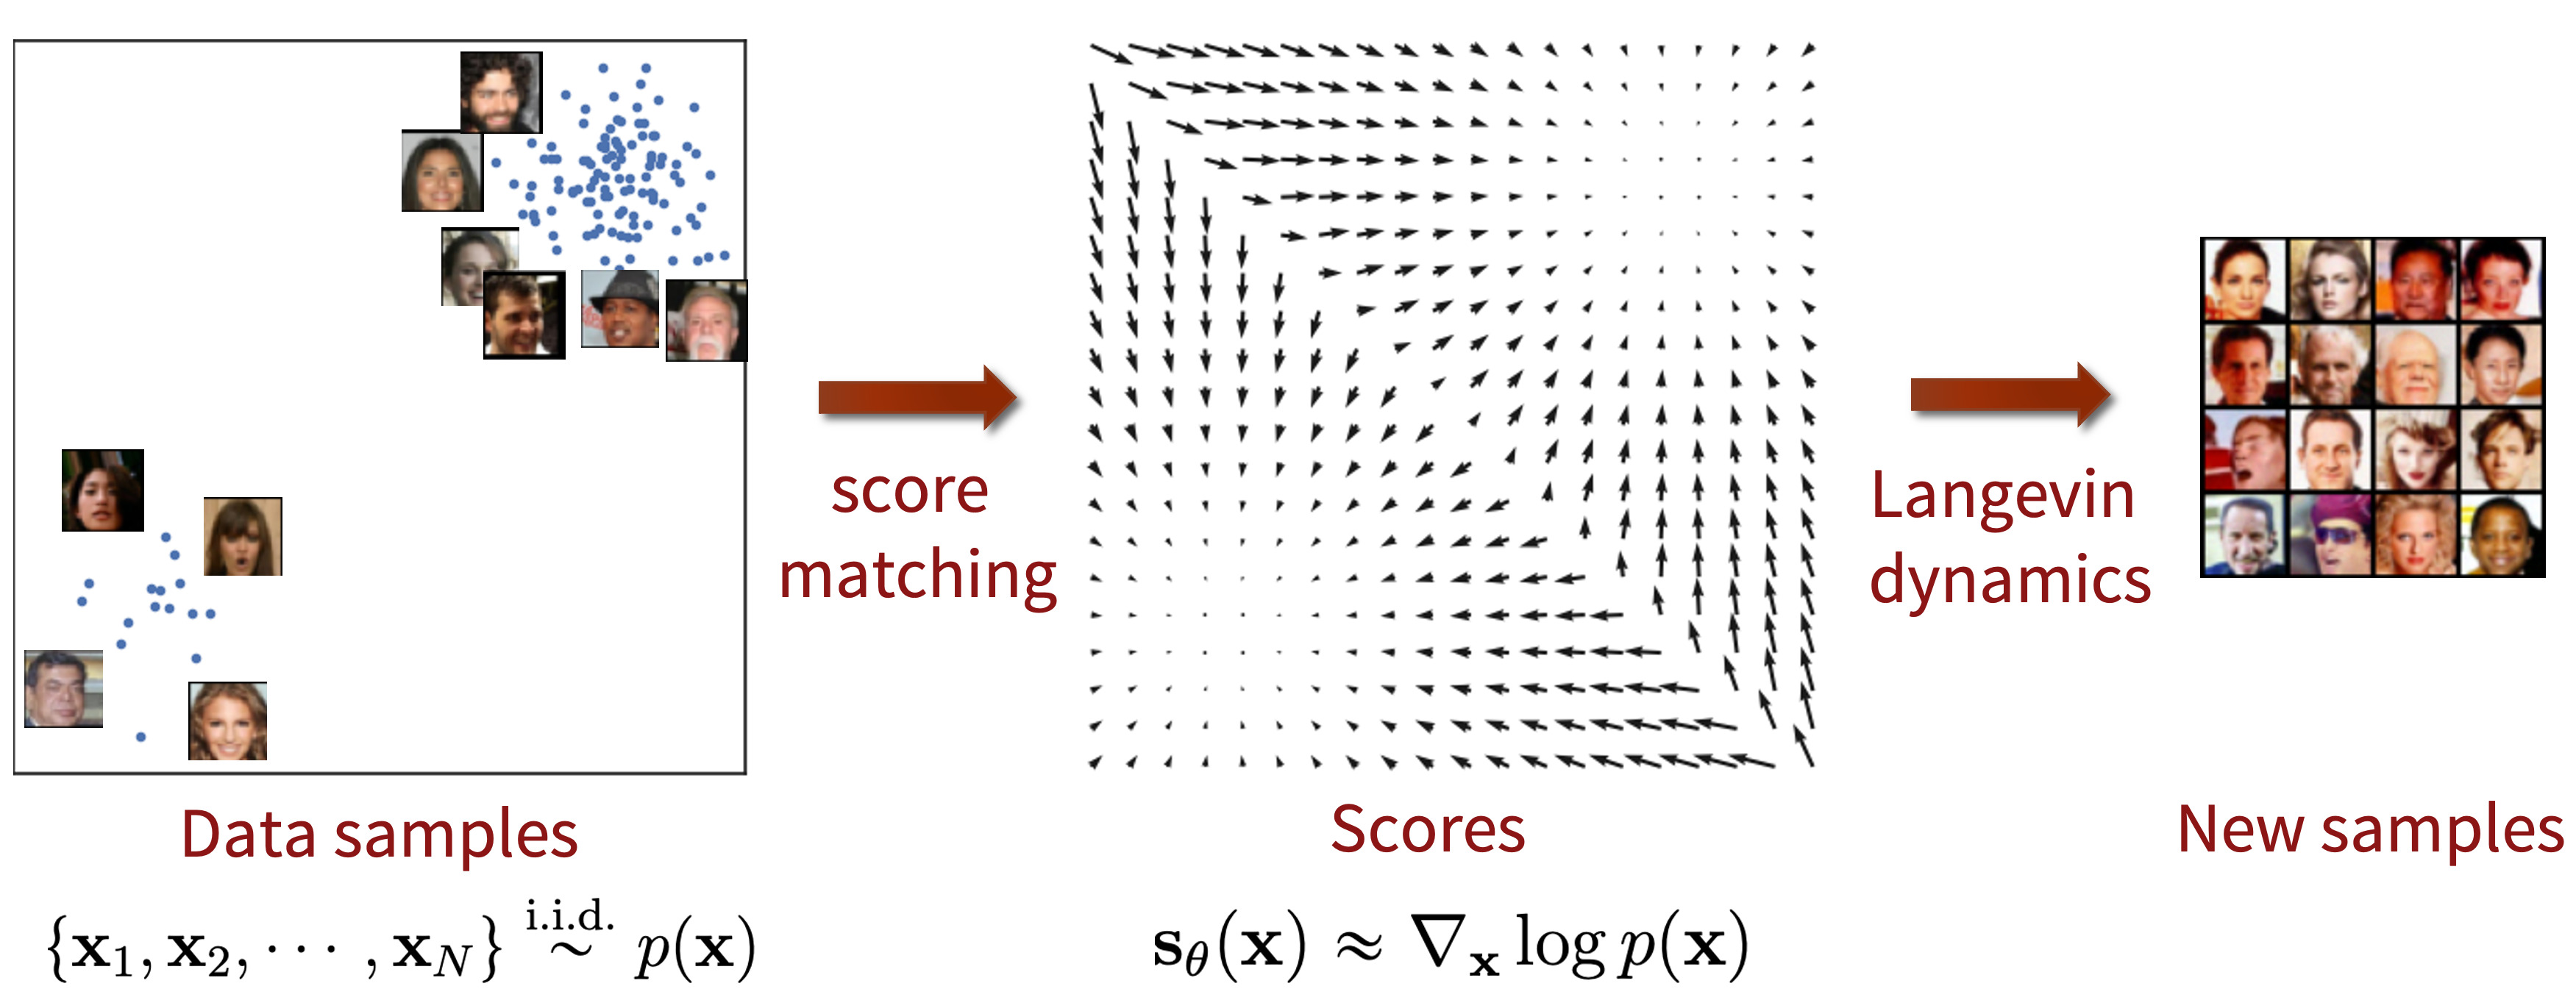
\includegraphics[width=0.75\linewidth]{figs/smld}
	\end{figure}
	\vspace{-0.3cm} 
	\textbf{Problem:} we do not know $\nabla_\bx \log \pi(\bx)$.
	\myfootnotewithlink{https://yang-song.github.io/blog/2021/score/}{Song Y. Generative Modeling by Estimating Gradients of the Data Distribution, blog post, 2021}
\end{frame}
%=======
\section{Denoising score matching}
%=======
\begin{frame}{Denoising score matching}
	Let perturb original data $\bx \sim \pi(\bx)$ by random normal noise 
	\[
		\bx' = \bx + \sigma \cdot \bepsilon, \quad \bepsilon \sim \cN(0, \bI), \quad p(\bx' | \bx, \sigma) = \cN(\bx' | \bx, \sigma^2 \bI)
	\]
	\vspace{-0.4cm}
	\[
		\pi(\bx' | \sigma) = \int p(\bx' | \bx, \sigma) \pi(\bx) d\bx.
	\]
	\vspace{-0.4cm} 
	\begin{block}{Assumption}
		The solution of 
		\[
			\frac{1}{2} \bbE_{\pi(\bx' | \sigma)}\bigl\| \bs_{\btheta}(\bx', \sigma) - \nabla_{\bx'} \log \pi(\bx' | \sigma) \bigr\|^2_2 \rightarrow \min_{\btheta}
		\]
		\vspace{-0.3cm} \\
		satisfies $\bs_{\btheta}(\bx', \sigma) \approx \bs_{\btheta}(\bx', 0) = \bs_{\btheta}(\bx)$ if $\sigma$ is small enough.
	\end{block}
	\begin{itemize}
		\item $\bs_{\btheta}(\bx', \sigma)$ tries to \textbf{denoise} a corrupted sample $\bx'$.
		\item Score function $\bs_{\btheta}(\bx', \sigma)$ parametrized by $\sigma$. 
	\end{itemize}
	\myfootnotewithlink{http://www.iro.umontreal.ca/~vincentp/Publications/smdae_techreport.pdf}{Vincent P. A Connection Between Score Matching and Denoising Autoencoders, 2010}
\end{frame}
%=======
\begin{frame}{Denoising score matching}
	\begin{block}{Theorem}
	\vspace{-0.5cm}
	\begin{multline*}
		\bbE_{\pi(\bx' | \sigma)}\bigl\| \bs_{\btheta}(\bx', \sigma) - \nabla_{\bx'} \log \pi(\bx' | \sigma) \bigr\|^2_2 = \\
		= \bbE_{\pi(\bx)} \bbE_{p(\bx' | \bx, \sigma)}\bigl\| \bs_{\btheta}(\bx', \sigma) - \nabla_{\bx'} \log p(\bx' | \bx, \sigma) \bigr\|^2_2 + \text{const}(\btheta)
	\end{multline*}
	\vspace{-0.5cm}
	\end{block}
	\begin{block}{Proof}
		\vspace{-0.7cm}
		{\small
		\begin{multline*}
			\bbE_{\pi(\bx' | \sigma)}\bigl\| \bs_{\btheta}(\bx', \sigma) - \nabla_{\bx'} \log \pi(\bx' | \sigma) \bigr\|^2_2 = \\ 
			= \bbE_{\pi(\bx' | \sigma)} \Bigl[\| {\color{olive}\bs_{\btheta}(\bx', \sigma) \|^2} + \underbrace{\| \nabla_{\bx'} \log \pi(\bx' | \sigma) \|^2_2}_{\text{const}(\btheta)} - 2 \bs_{\btheta}^T(\bx', \sigma) \nabla_{\bx'} \log \pi(\bx' | \sigma) \Bigr]
		\end{multline*}
		\vspace{-0.7cm}
		\begin{multline*}
			\bbE_{\pi(\bx' | \sigma)} {\color{olive} \| \bs_{\btheta}(\bx', \sigma) \|^2} = \int {\color{violet}\pi(\bx' | \sigma)} \| \bs_{\btheta}(\bx', \sigma) \|^2 d\bx' = \\
			= \int \left({\color{violet}\int p(\bx' | \bx, \sigma) \pi(\bx) d\bx}\right) \| \bs_{\btheta}(\bx', \sigma) \|^2 d\bx' =  \bbE_{\pi(\bx)} \bbE_{p(\bx' | \bx, \sigma)}  \| \bs_{\btheta}(\bx', \sigma) \|^2 d\bx'
		\end{multline*}
		}
	\end{block}
	\myfootnotewithlink{http://www.iro.umontreal.ca/~vincentp/Publications/smdae_techreport.pdf}{Vincent P. A Connection Between Score Matching and Denoising Autoencoders, 2010}
\end{frame}
%=======
\begin{frame}{Denoising score matching}
	\begin{block}{Theorem}
	\vspace{-0.5cm}
	\begin{multline*}
		\bbE_{\pi(\bx' | \sigma)}\bigl\| \bs_{\btheta}(\bx', \sigma) - \nabla_{\bx'} \log \pi(\bx' | \sigma) \bigr\|^2_2 = \\
		= \bbE_{\pi(\bx)} \bbE_{p(\bx' | \bx, \sigma)}\bigl\| \bs_{\btheta}(\bx', \sigma) - \nabla_{\bx'} \log p(\bx' | \bx, \sigma) \bigr\|^2_2 + \text{const}(\btheta)
	\end{multline*}
	\vspace{-0.5cm}
	\end{block}
	\begin{block}{Proof (continued)}
		\vspace{-0.7cm}
		{\small
		\begin{multline*}
			\bbE_{\pi(\bx' | \sigma)} \left[{\color{teal}\bs_{\btheta}^T(\bx', \sigma) \nabla_{\bx'} \log \pi(\bx' | \sigma)} \right] = \int \pi(\bx' | \sigma) \left[\bs_{\btheta}^T(\bx', \sigma) \frac{\nabla_{\bx'} {\color{violet}\pi(\bx' | \sigma)}}{\pi(\bx' | \sigma)} \right] d \bx' = \\
			= \int \left[\bs_{\btheta}^T(\bx', \sigma) \nabla_{\bx'}\left({\color{violet}\int p(\bx' | \bx, \sigma) \pi(\bx) d\bx}\right) \right] d \bx' = \\
			=  \int \int \pi(\bx) \left[\bs_{\btheta}^T(\bx', \sigma) {\color{olive}\nabla_{\bx'}p(\bx' | \bx, \sigma)} \right] d \bx' d\bx = \\
			= \int \int \pi(\bx) {\color{olive} p(\bx' | \bx, \sigma)} \left[\bs_{\btheta}^T(\bx', \sigma) {\color{olive}\nabla_{\bx'} \log p(\bx' | \bx, \sigma)} \right] d \bx' d\bx = \\
			= \bbE_{\pi(\bx)} \bbE_{p(\bx' | \bx, \sigma)} \left[{\color{teal}\bs_{\btheta}^T(\bx', \sigma) \nabla_{\bx'} \log p(\bx' | \bx, \sigma)} \right]
		\end{multline*}
		}
	\end{block}
	\myfootnotewithlink{http://www.iro.umontreal.ca/~vincentp/Publications/smdae_techreport.pdf}{Vincent P. A Connection Between Score Matching and Denoising Autoencoders, 2010}
\end{frame}
%=======
\begin{frame}{Denoising score matching}
	\begin{block}{Theorem}
	\vspace{-0.7cm}
	\begin{multline*}
		\bbE_{\pi(\bx' | \sigma)}\bigl\| \bs_{\btheta}(\bx', \sigma) - \nabla_{\bx'} \log \pi(\bx' | \sigma) \bigr\|^2_2 = \\
		= \bbE_{\pi(\bx)} \bbE_{p(\bx' | \bx, \sigma)}\bigl\| \bs_{\btheta}(\bx', \sigma) - \nabla_{\bx'} \log p(\bx' | \bx, \sigma) \bigr\|^2_2 + \text{const}(\btheta)
	\end{multline*}
	\vspace{-0.9cm}
	\end{block}
	\begin{block}{Proof (continued)}
		\vspace{-0.7cm}
		{\small
		\begin{multline*}
			\bbE_{\pi(\bx' | \sigma)}\bigl\| \bs_{\btheta}(\bx', \sigma) - \nabla_{\bx'} \log \pi(\bx' | \sigma) \bigr\|^2_2 = \\ 
			= {\color{olive}\bbE_{\pi(\bx' | \sigma)}} \Bigl[\| \bs_{\btheta}(\bx', \sigma) \|^2 - 2 \bs_{\btheta}^T(\bx', \sigma) {\color{teal}\nabla_{\bx'} \log \pi(\bx' | \sigma)} \Bigr] + \text{const}(\btheta) = \\
			= {\color{olive}\bbE_{\pi(\bx)} \bbE_{p(\bx' | \bx, \sigma)}}\Bigl[\| \bs_{\btheta}(\bx', \sigma) \|^2 - 2 \bs_{\btheta}^T(\bx', \sigma) {\color{teal}\nabla_{\bx'} \log p(\bx' | \bx, \sigma)} \Bigr] + \text{const}(\btheta)
		\end{multline*}
		}
		\vspace{-0.8cm}
	\end{block}
	\begin{block}{Gradient of the noise kernel}
	\vspace{-0.4cm}
	\[
		\nabla_{\bx'} \log p(\bx' | \bx, \sigma) = \nabla_{\bx'} \log \cN(\bx' | \bx, \sigma^2 \bI) = - \frac{\bx' - \bx}{\sigma^2}
	\]
	\vspace{-0.5cm}
	\end{block}
	The RHS does not need to compute $\nabla_{\bx'} \log \pi(\bx' | \sigma)$ and even $\nabla_{\bx'} \log \pi(\bx')$.
	\myfootnotewithlink{http://www.iro.umontreal.ca/~vincentp/Publications/smdae_techreport.pdf}{Vincent P. A Connection Between Score Matching and Denoising Autoencoders, 2010}
\end{frame}
%=======
\begin{frame}{Denoising score matching}
	\begin{itemize}
		\item If $\sigma$ is \textbf{small}, the score function is not accurate and Langevin dynamics will probably fail to jump between modes.
		\begin{figure}
			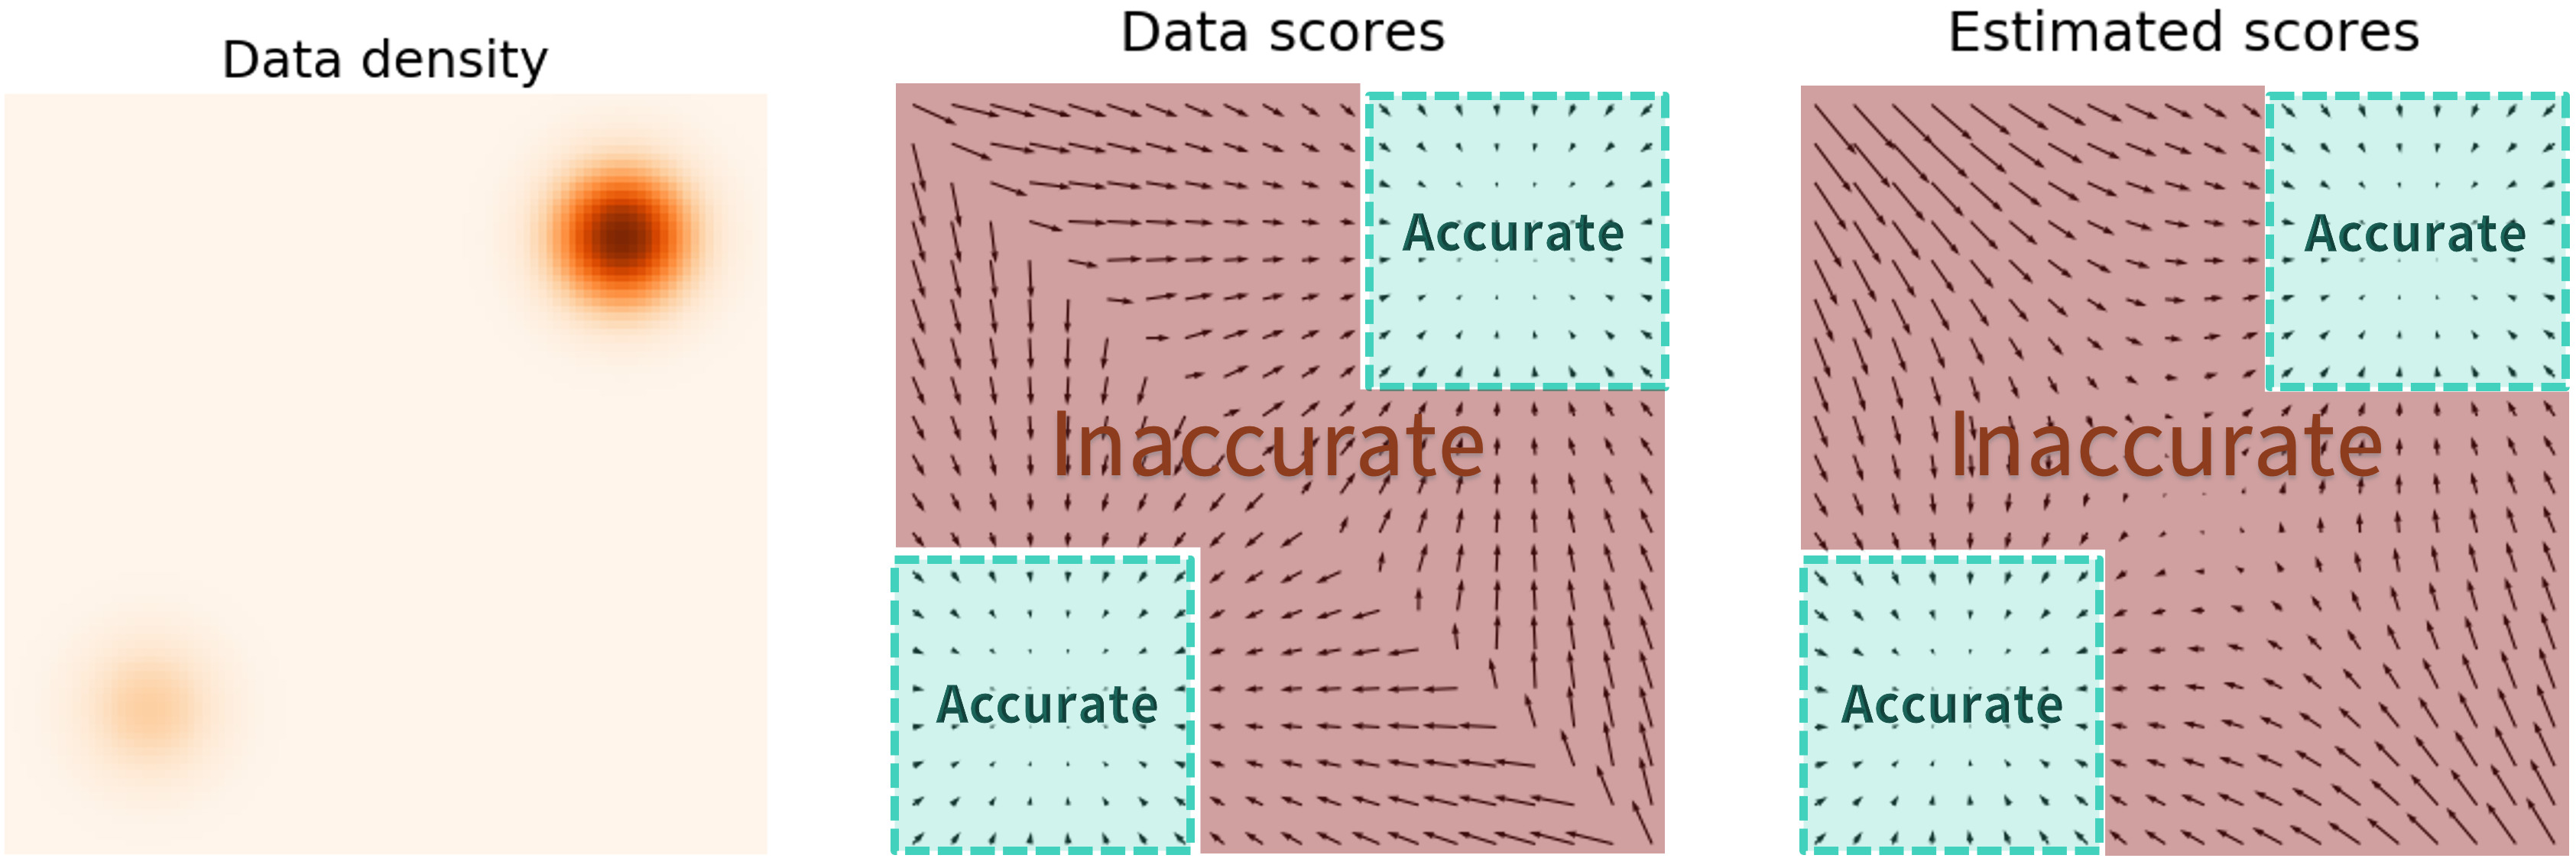
\includegraphics[width=0.75\linewidth]{figs/pitfalls}
		\end{figure}
		\item If $\sigma$ is \textbf{large}, it is good for low-density regions and  multimodal distributions, but we will learn too corrupted distribution.
		\begin{figure}
			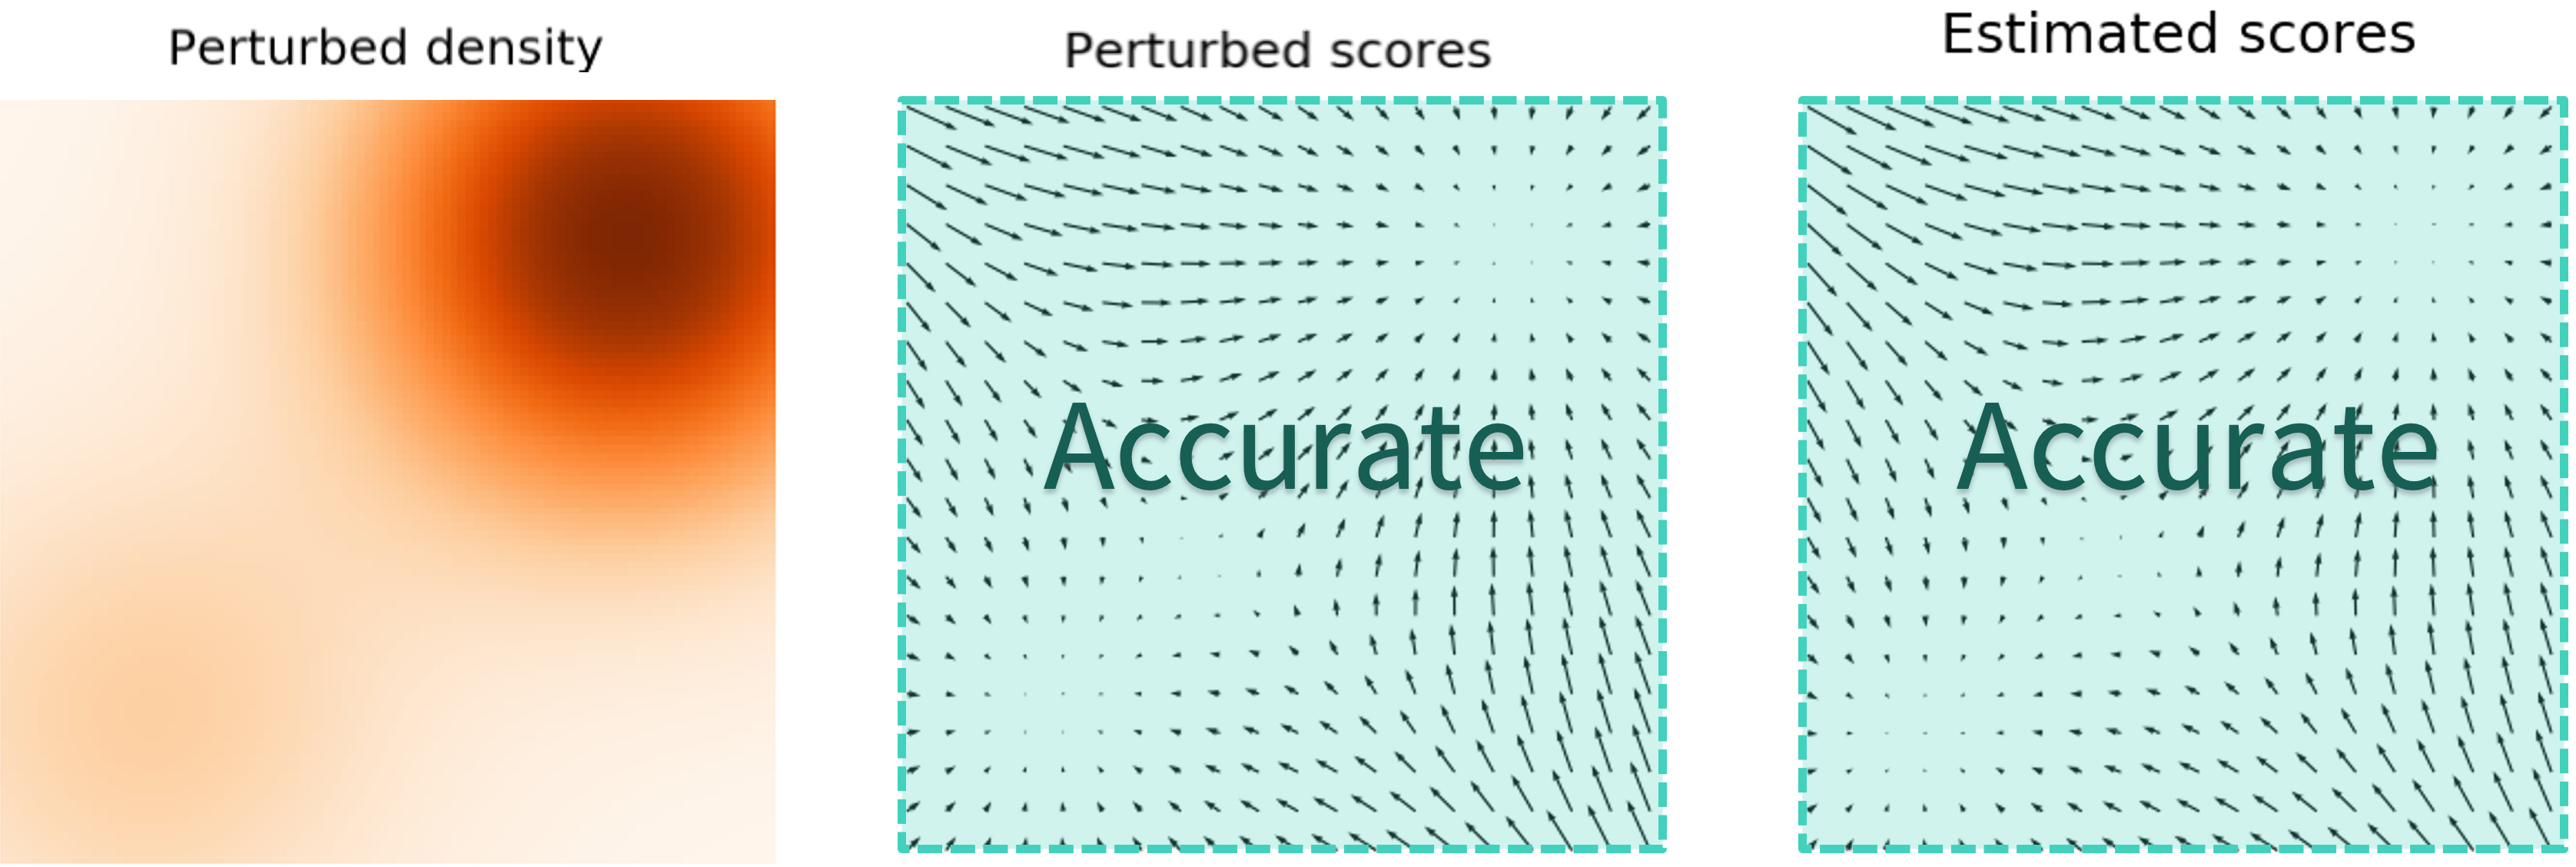
\includegraphics[width=0.75\linewidth]{figs/single_noise}
		\end{figure}
	\end{itemize}
	\myfootnotewithlink{https://yang-song.github.io/blog/2021/score/}{Song Y. Generative Modeling by Estimating Gradients of the Data Distribution, blog post, 2021}
\end{frame}
%=======
\section{Noise Conditioned Score Network (NCSN)}
%=======
\begin{frame}{Noise Conditioned Score Network (NCSN)}
	\begin{itemize}
		\item Define the sequence of the noise levels: $\sigma_1 > \sigma_2 > \dots > \sigma_L$.
		\item Perturb the original data with the different noise levels to obtain $\pi(\bx' | \sigma_1), \dots, \pi(\bx' | \sigma_L)$.
		\item Choose $\sigma_1, \sigma_L$ such that:
		\[
			\pi(\bx' | \sigma_1) \approx \cN(0, \sigma_1^2 \bI), \quad \pi(\bx' | \sigma_L) \approx \pi(\bx).
		\]
	\end{itemize}
	\begin{figure}
		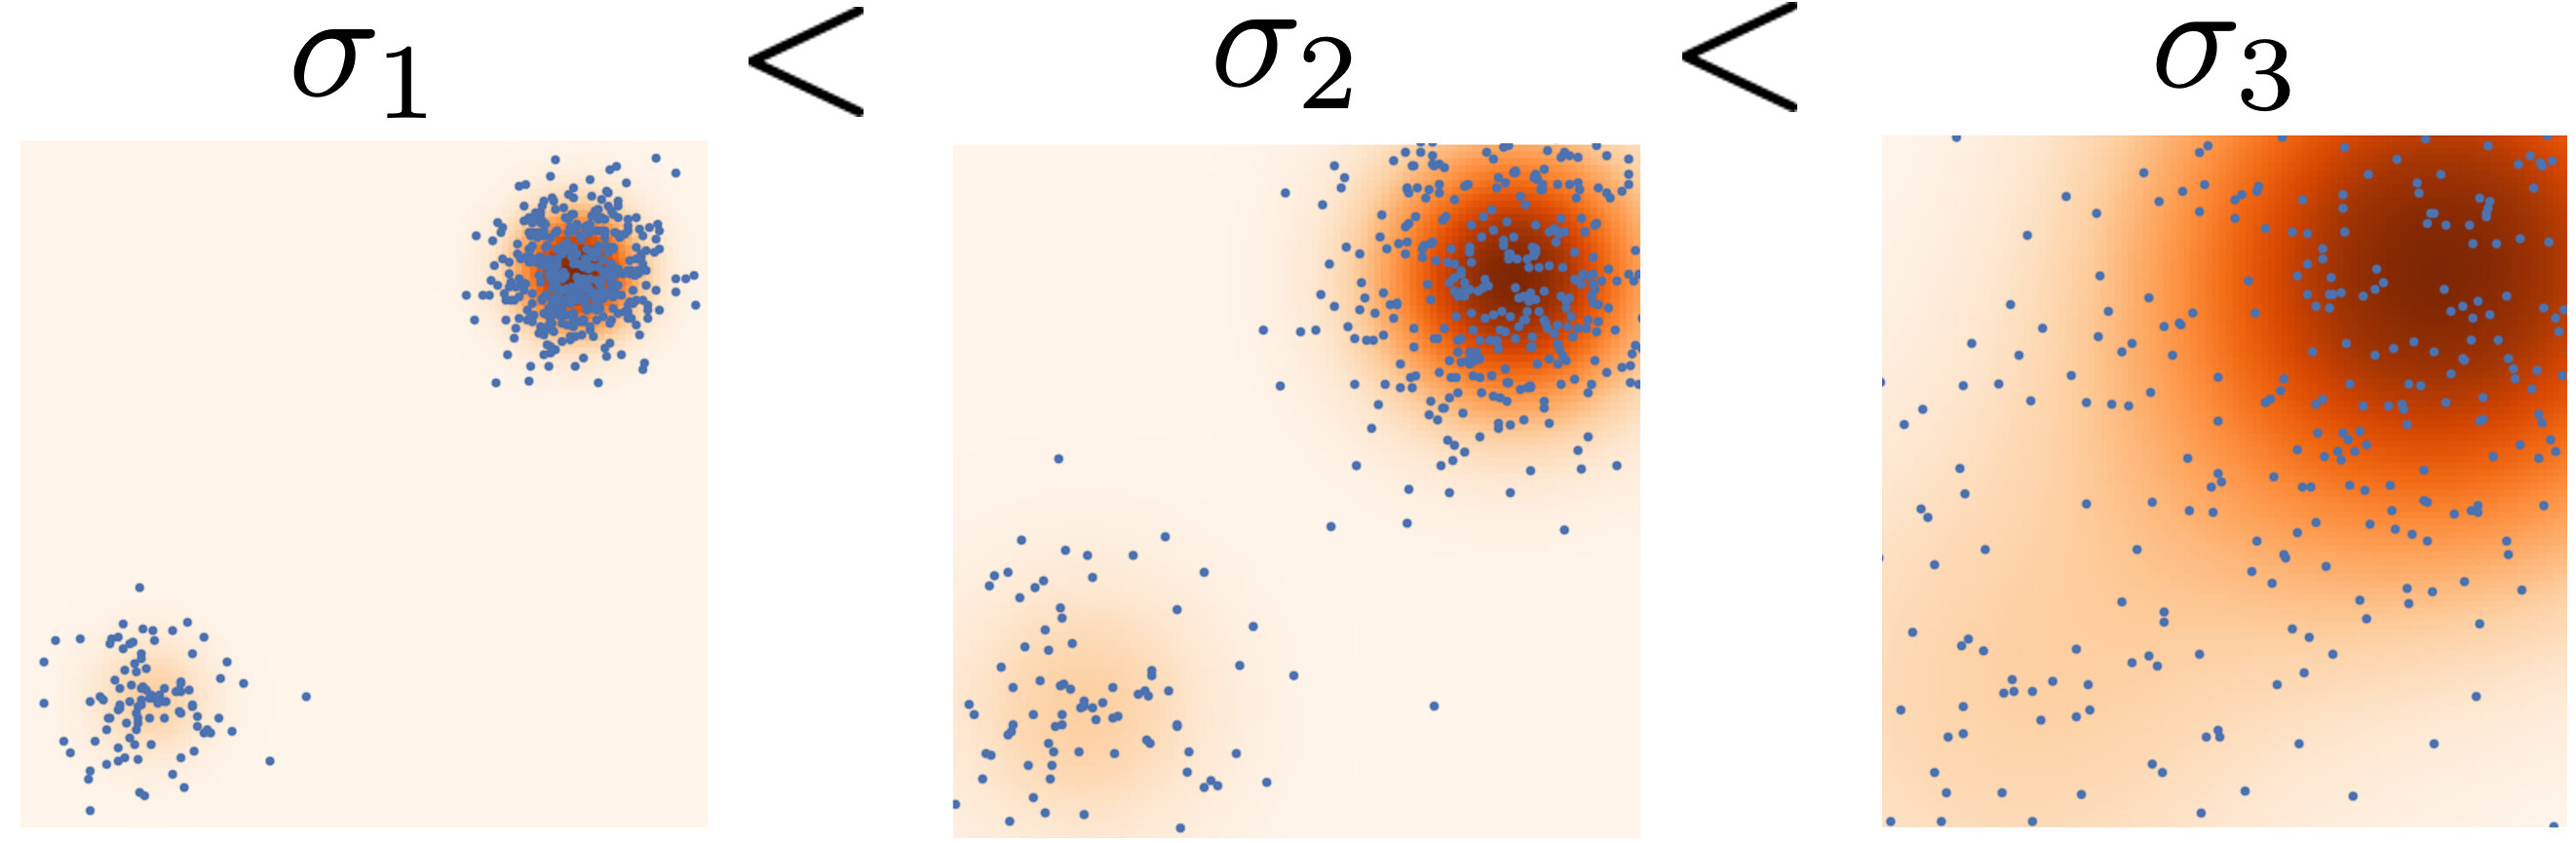
\includegraphics[width=0.6\linewidth]{figs/multi_scale}
	\end{figure}
	\begin{figure}
		
\includegraphics[width=\linewidth]{figs/duoduo}
	\end{figure}
	\myfootnotewithlink{https://arxiv.org/abs/1907.05600}{Song Y. et al. Generative Modeling by Estimating Gradients of the Data Distribution, 2019}
\end{frame}
%=======
\begin{frame}{Noise Conditioned Score Network (NCSN)}
	Train the denoising score function $\bs_{\btheta}(\bx', \sigma)$ for each noise level using unified weighted objective:
	\vspace{-0.2cm}
	\[
		\sum_{l=1}^L {\color{violet}\sigma_l^2} \bbE_{\pi(\bx)} \bbE_{p(\bx' | \bx, \sigma_l)}\bigl\| \bs_{\btheta}(\bx', \sigma_l) - \nabla_{\bx'} \log p(\bx' | \bx, \sigma_l) \bigr\|^2_2 \rightarrow \min_{\btheta}
	\]
	Here $\nabla_{\bx'} \log p(\bx' | \bx, \sigma_l) = - \frac{\bx' - \bx}{\sigma_l^2} = - \frac{\bepsilon}{\sigma_l}$.
	\begin{block}{Training}
		\begin{enumerate}
			\item Get the sample $\bx_0 \sim \pi(\bx)$.
			\item Sample noise level $l \sim U[1, L]$ and the noise $\bepsilon \sim \cN(0, \bI)$.
			\item Get noisy image $\bx' = \bx_0 + \sigma_l \cdot \bepsilon$.
			\item Compute loss $ \cL = \| \bs_{\btheta}(\bx', \sigma_l) + \frac{\bepsilon}{\sigma_l} \|^2 $.
		\end{enumerate}
	\end{block}
	How to sample from this model?
	\myfootnotewithlink{https://arxiv.org/abs/1907.05600}{Song Y. et al. Generative Modeling by Estimating Gradients of the Data Distribution, 2019}
\end{frame}
%=======
\begin{frame}{Noise Conditioned Score Network (NCSN)}
	\begin{block}{Sampling (annealed Langevin dynamics)}
		\begin{itemize}
			\item Sample $\bx_0 \sim \cN(0, \sigma_1 \bI) \approx \pi(\bx | \sigma_1)$.
			\item Apply $T$ steps of Langevin dynamic
			\vspace{-0.2cm}
			\[
				\bx_t = \bx_{t-1} + \frac{1}{2}\eta_l \bs_{\btheta}(\bx_{t - 1}, \sigma_l) + \sqrt{\eta_l} \bepsilon_t.
			\] 
			\vspace{-0.5cm}
			\item Update $\bx_0 := \bx_T$ and choose the next $\sigma_l$.
		\end{itemize}
	\end{block}
	\begin{figure}
		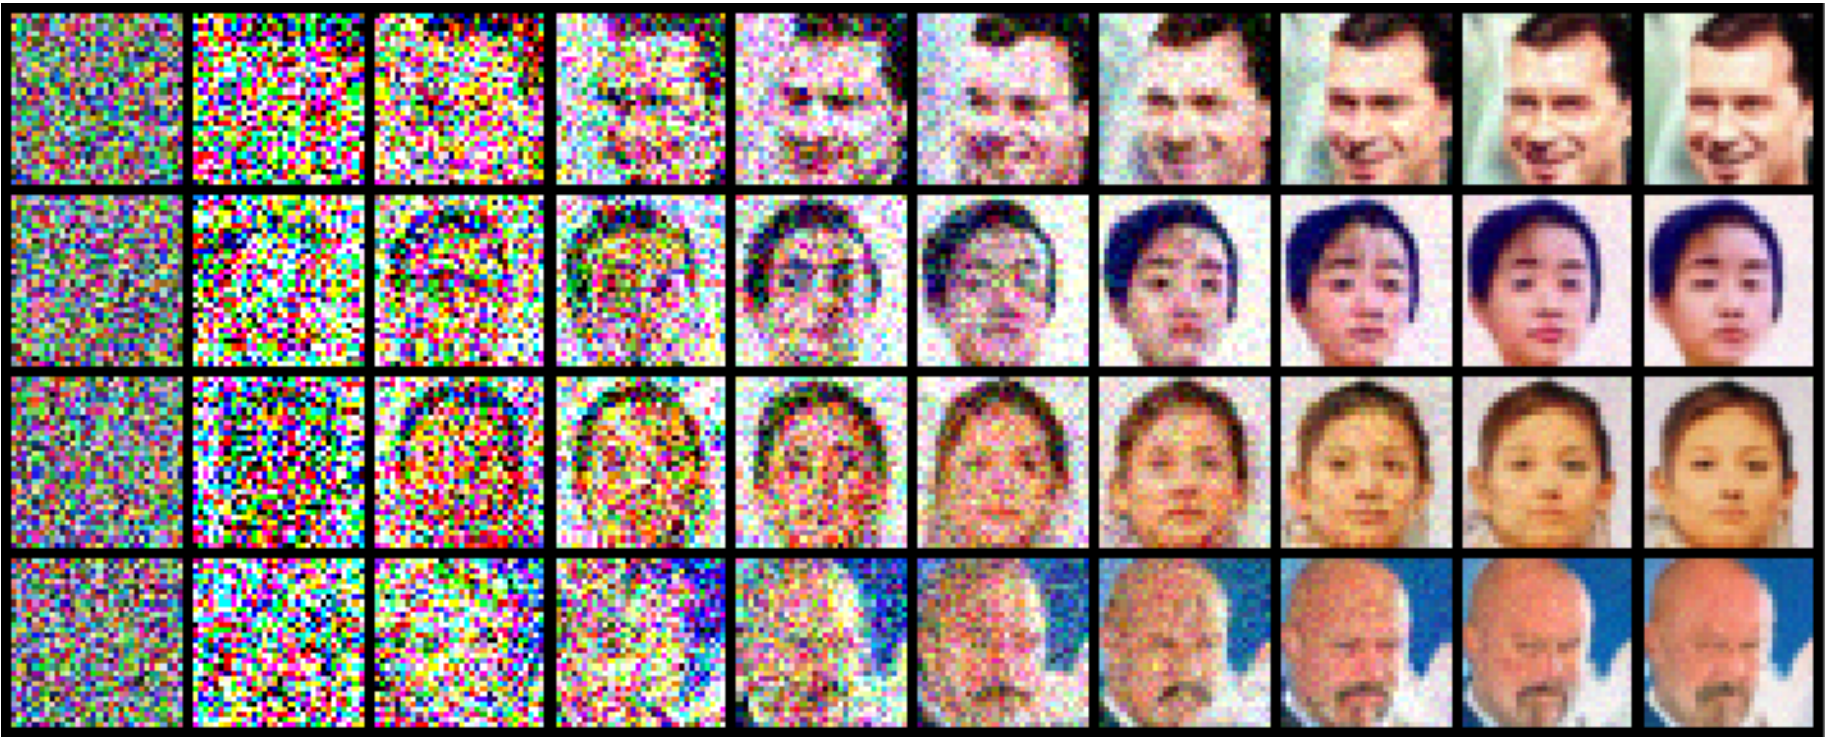
\includegraphics[width=0.9\linewidth]{figs/ald}
	\end{figure}
	\myfootnotewithlink{https://arxiv.org/abs/2006.09011}{Song Y. et al. Improved Techniques for Training Score-Based Generative Models, 2020}
\end{frame}
%=======
\begin{frame}{Summary}
	\begin{itemize}
		\item Langevin dynamics allows to sample from the generative model using the gradient of the log-likelihood.	
		\vfill
		\item Score matching proposes to minimize Fisher divergence to get the score function.
		\vfill
		\item Denoising score matching minimizes Fisher divergence on noisy samples. It allows to estimate Fisher divergence using samples.
		\vfill
		\item Noise conditioned score network uses multiple noise levels and annealed Langevin dynamics to fit score function and sample from the model.
	\end{itemize}
\end{frame}
\end{document} 